\documentclass[10pt,twocolumn,letterpaper]{article} 

\usepackage{avss}
\usepackage{times}
\usepackage{epsfig}
\usepackage{graphicx}
\usepackage{amsmath}
\usepackage{amssymb}


\usepackage[colorlinks,
linkcolor=red,
anchorcolor=blue,
citecolor=green
]{hyperref}


% Include other packages here, before hyperref.

% If you comment hyperref and then uncomment it, you should delete 
% egpaper.aux before re-running latex.  (Or just hit 'q' on the first latex
% run, let it finish, and you should be clear).
%\usepackage[pagebackref=true,breaklinks=true,letterpaper=true,colorlinks,bookmarks=false]{hyperref}


%\avssfinalcopy % *** Uncomment this line for the final submission

\def\avssPaperID{21} % *** Enter the AVSS Paper ID here
\def\httilde{\mbox{\tt\raisebox{-.5ex}{\symbol{126}}}}

% Pages are numbered in submission mode, and unnumbered in camera-ready
\ifavssfinal\pagestyle{empty}\fi
\begin{document}

%%%%%%%%% TITLE
\title{Efficient 3D Convolutional Neural Networks for Violence Detection}

\author{First Author\\
Institution1\\
Institution1 address\\
{\tt\small firstauthor@i1.org}
% For a paper whose authors are all at the same institution, 
% omit the following lines up until the closing ``}''.
% Additional authors and addresses can be added with ``\and'', 
% just like the second author.
% To save space, use either the email address or home page, not both
\and
Second Author\\
Institution2\\
First line of institution2 address\\
{\tt\small secondauthor@i1.org}
}

\maketitle
% \thispagestyle{empty}

%%%%%%%%% ABSTRACT
\begin{abstract}
Automatically analyzing violent content in surveillance videos is of profound significance on many applications, ranging from video content filtration to public security protection. Recognition accuracy and computational efficiency are two key factors to perform this task. In this paper, we propose a deep learning model based on 3D convolutional neural networks with improved internal architecture, which is more capable of capturing spatiotemporal features and requires relatively fewer parameters. The proposed model is validated on three standard datasets in terms of classification accuracy. Meanwhile, supplementary experiment is carried out to evaluate its effectiveness and efficiency. The final results demonstrate the advantages of our model over the state-of-the-art approaches in both recognition accuracy and computational efficiency.
\end{abstract}

%%%%%%%%% BODY TEXT
\section{Introduction} \label{sec:1}

Nowadays, violence and terrorist attack have become primary threats to world security and stability.
Thanks to the development of digital media technologies, violent scenes can be recorded by surveillance cameras.
However, with a large number of video materials produced every moment, it is unrealistic to manually guard these videos and capture every violent scene in real time.
Consequently, it is of profound significance to develop an efficient system which can automatically monitor and detect violence in surveillance videos.
In current tasks, violence is considered as aggressive behaviors of human, rather than fire, shots, explosion or blood.
Based on the above conception, there are three standard benchmark datasets constructed for performance evaluation.
We follow the meaning of violence in this work to keep consistent with related researches.

In recent years, computer vision has been continuing to evolve with the improvement of computing power and the availability of large-scale datasets.
Deep learning, a critical technology in computer vision, has achieved remarkable milestone in many fields, such as image classification and object detection.
It has also been introduced to address the problem of violence detection in videos.
Compared to approaches based on hand-crafted features, deep learning methods yield tremendous improvements in robustness and recognition accuracy.
However, there may be trade-offs and hard choices when considering both computational efficiency and recognition accuracy.
Consequently, developing an effective and efficient deep learning model is very crucial in practical applications.

Considering this situation, we leverage the latest research findings in computer vision and develop a deep neural networks for violence detection. Our major contributions are summarized as follows:
\begin{itemize}
	\item We propose a deep learning model based on 3D ConvNets with improved internal architecture for violence detection tasks.
	\item We demonstrate that properly selected internal architectures can improve the ability of representing abstract spatiotemporal information and reducing the number of parameters.
	\item We experimentally validate our model on three standard benchmark datasets and conduct supplementary experiment to evaluate the effectiveness and efficiency of our model.
\end{itemize}

The rest of the paper is organized as follows: Section 2 introduces the related works and approaches for violence detection. Section 3 explains the details of the proposed method, followed by experiment and analysis in Section 4. Finally, Section 5 concludes the work in this paper.

%------------------------------------------------------------------------

\section{Related Works}

At early stage of research, violence detection approaches \cite{nam1998audio, cheng2003semantic, zajdel2007cassandra} generally rely on the detection of specific visual cues such as flame, blood and explosion together with audio content like gunshot or breaking sound.

To reduce this impact, Zajdel et al. \cite{zajdel2007cassandra} present a surveillance system, exploiting of the complimentary nature of audio and video.
Acar et al. \cite{acar2016breaking} use time efficient audio features in coarse-level analysis and use advanced motion features to pursue fine-level analysis when necessary.
In practical scenarios, however, most of the surveillance cameras do not contain any audio devices, resulting in the fact that  the majority of video contents do not have audio tracks, which brings great difficulties to audio-based methods. 
As a result, methods based on video contents become the mainstream. 

Video-based violence detection can be divided into two categories according to their feature extraction methods:
traditional hand-crafted feature based methods, and deep learning methods.

Hand-crafted feature based approaches, generally, extract relatively robust features designed by human, then aggregate these features with encoding strategies, and apply machine learning classifiers for the final decision.
Among these methods, STIP \cite{STIPs}, MoSIFT \cite{MoSIFT} and iDT \cite{iDTs} descriptors are widely used features in violence detection tasks such as \cite{vio_sift, hockey, mosift_sc}.
Hassner et al. \cite{vif} propose a novel feature descriptor, namely VIolent Flows (ViF), by considering the statistics of optical flow vector magnitude changes over time. They also introduce VIolent Flows benchmark dataset in their work.
Later, Gao et al. \cite{ovif} improve this method and take full advantage of the motion magnitude change information by calculating the histograms of oriented optical flow, resulting in Oriented VIolent Flows (OViF) feature.
A fast detection method is proposed by Deniz et al. in \cite{fast}, with extreme accelerations efficiently estimated by applying the Radon transform to the power spectrum of consecutive frames.
Mohammadi et al. \cite{moha_avss} exploit the spatiotemporal characteristic of substantial derivative, an important concept in fluid mechanics, as feature extraction for violence detection.
Gracia et al. \cite{blob} use features extracted from motion blobs to discriminate fight and non-fight sequences. 
Zhang et al. \cite{MoIWLD} propose a modified motion Weber local descriptor (MoIWLD), integrated with the sparse representation, as the new feature descriptor.
Senst et al. \cite{lagrangian} present a new feature using Lagrangian direction fields, where appearance, background motion compensation, and long-term motion information are used.
Deb et al. \cite{vlad} introduce a higher order statistics-based feature encoding method, called Outlier-Resistant VLAD (OR-VLAD), to improve the original VLAD performance.

Deep learning approaches aim to develop end-to-end trainable models including feature extraction, encoding, and classification. 
Simonyan et al. \cite{two-stream} first propose two-stream architecture for human action recognition, with spatial and temporal networks fusion by SVM, trying to capture motion information between frames using optical flow as input.
Dong et al. \cite{dong2016multi} extend this method to multi-stream, adding another acceleration stream for capturing the important intense information in violence. Also, they add LSTM \cite{lstm} before the final fusion to model long-term information.  
Zhou et al. \cite{zhou2017violent} borrow the idea from temporal segment networks (TSN) \cite{tsn} and propose a model named FightNet. They use RGB images, optical flow and acceleration field as input, and then fusion them with SoftMax.
Meng et al. \cite{meng2017trajectory} take the advantage of hand-crafted features, using improved trajectories and trajectory pooling in model for encoding long-term informations.
Serrano et al. \cite{serrano2018fight} use Hough Forests as feature extractor to build a representative image for each sequence, followed by 2DCNN for the final decision.
These methods leverage the hand-crafted features by combining them with deep learning models. However, there are some drawbacks. They are not actually end-to-end trainable as they take hand-crafted features as inputs. As a result, it may be inefficient to add additional computation.

Some other methods have been proposed to solve these problems.
Ding et al. \cite{3dcnn_ding} propose a 3D ConvNets model for violence detection without using any hand-crafted feature or prior knowledge. 
Sudhakaran et al. \cite{convlstm_sudh} use 2DCNN to extract spatial feature maps, followed by ConvLSTM \cite{convlstm} to encode spatiotemporal information, which is also end-to-end trainable.

%------------------------------------------------------------------------- 

% figures

\begin{figure*}
\begin{center}
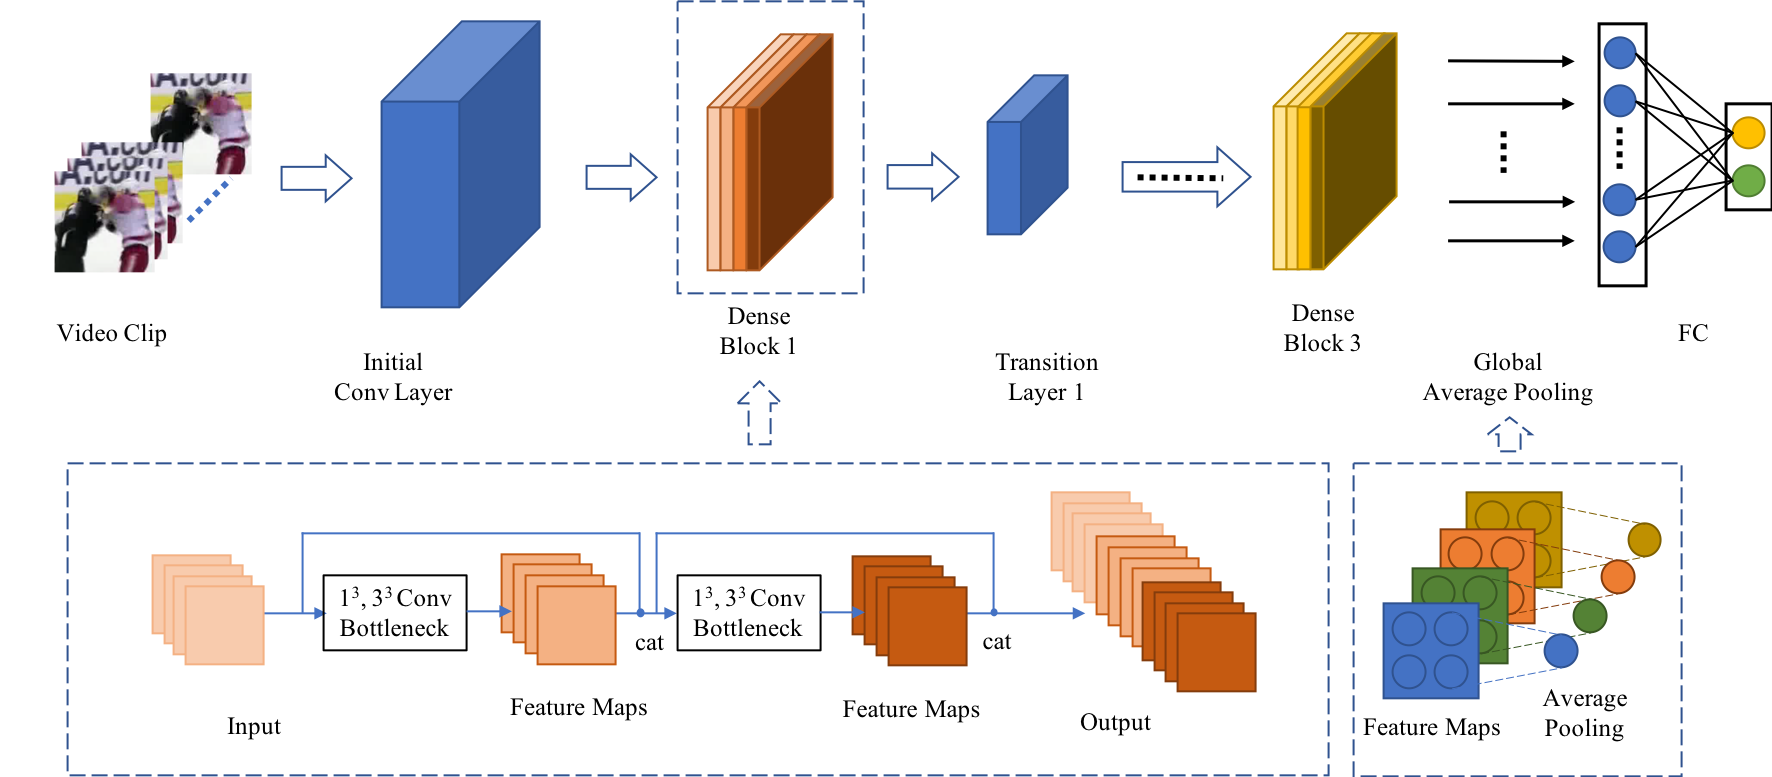
\includegraphics[scale=0.55]{fig/fig1.png}
\end{center}
\caption{Network architecture of proposed method. The model is composed of three dense blocks, two transition layers, one initial convolution layer and one fully connected layer (Dense Block 2 and Transition Layer 2 are omitted). Each dense block contains densely connected dense layers. The fully-connected layer are joined with output feature maps using global averaging pooling strategy. Diagram in the left dashed box illustrates the simplified details in dense block, where the number of dense layers is 2 and the growth rate $k$ is 4.}
\label{fig:model}
\end{figure*}


%------------------------------------------------------------------------- 


Recently, deep learning approaches have achieved great successes in the field of action recognition, due to the development of deep learning technologies and the availability of large scale datasets. 
Tran et al. \cite{3dcnn_1} research the features learned by 3D ConvNets and propose four properties for an effective video descriptor: generic, compact, efficient and simple. 
Carreira et al. \cite{kinetics} build a large-scale dataset called Kinetics, for human action recognition, which is similar to the role that ImageNet \cite{imagenet} dataset plays in image classification. 
Following this, Hara et al. \cite{3dcnn_2} perform a series of experiments and prove that 3D CNN and Kinetics dataset can have the potential contribution to the field of action recognition.
Tran et al. \cite{r2+1d} explore different kinds of 3D CNN architecture and design a new spatiotemporal convolutional block "R(2+1)D" for action recognition, achieving comparable or superior results.

By taking the advanced theory and practical experience above, we have developed an efficient and effective model based on 3D CNN with special designed architecture for violence detection tasks.

%------------------------------------------------------------------------- 

\section{Proposed Method}
Our aim is to design a deep neural network model for classifying fight and non-fight clips from RGB videos. 
For a system able to identify violent scenes, it should be capable of capturing the motion of human body over time. 
Recognition accuracy and computational efficiency are two important indicators of this task.
Consequently, it is of great importance to developing an effective and efficient spatiotemporal feature extractor module.
In view of these facts, we follow the conclusion and advice in \cite{3dcnn_1, r2+1d} and refer to the success of DenseNet \cite{densenet} architecture, and finally develop an efficient and effective model based on 3D convolutional networks.


\subsection{Rethinking 3D Convolutional Networks}

For a video classification task, the most critical issue is to extract appropriate features which are representative for the video content.
Compared to other architectures, 3D ConvNets can effectively capture spatiotemporal features  with convolution kernel extended to three dimensions. 
It implies that there is no need to apply LSTM or other RNN architecture for temporal information encoding. 
Also raw pixels are taken as input without complex preprocessing or extra calculation, as is much more computational efficient than other deep learning model using optical flow, trajectories etc.

However, the number of parameters may be exponentially increased due to the characteristics of 3D convolution itself, which may bring two main problems: 
Firstly, more parameters require higher FLOPs, which is computational inefficient; 
Secondly, redundant parameters may cause model overfitting and decreasing in generalization, especially in small dataset. 
To solve these problems and promote 3D ConvNets to give scope to feature representation, we take advantages of latest research findings.

The most direct approach is trying to reduce the size of convolution kernel. For example, two serialized 3$\times$3$\times$3 kernels nearly have the same representational ability of one 5$\times$5$\times$5 kernel, while the number of parameters is only the half. And it has been found and suggested in \cite{3dcnn_1} that 3$\times$3$\times$3 is the best kernel choice for 3D ConvNets.

Encouraging feature reusing is also a good practice in designing networks. In model training phase, it helps to facilitate the back propagation of information flow, which conduces to avoid overfitting and improve generalization. DenseNet \cite{densenet} gives a serials of inspirations on developing a compact but effective architecture.

\subsection{Network Architecture}

An overview of our model is illustrated in Figure \ref{fig:model}, including three dense blocks and two transition layers. 
All kernel sizes of convolutional layers and pooling layers are three-dimensional. 
The initial convolutional layer is a traditional convolutional layer with kernel size 7$\times$7$\times$7. 
Then these feature maps are used in the following first dense block. 
As is similar in \cite{densenet}, dense block is comprised of several dense layers, and these layers are directly connected with each other. 
The $l^{th}$ layer receives the output feature maps of all its preceding layers, $y_0$, $y_1$, $\cdots$, $y_{l-1}$, as inputs:
\begin{equation}
\label{eq:densenet}
y_l = H_l\left([y_0, y_1, \cdots, y_{l-1}]\right)
\end{equation}
where $H_l(*)$ is the state transition function of the $l^{th}$ layer, and $[*]$ denotes concatenating operation.
Each dense layer produces $k$ new feature maps, where $k$ is a hyper-parameter and is referred as growth rate. For a dense block containing $L$ layers, it produces $k \times L$ new feature maps.

At the end of this model, we use global average pooling strategy proposed in \cite{NinN} to bridge the convolutional structure with fully connected layer for classification.
As is illustrated in the right dashed box in Figure \ref{fig:model}, the final output feature maps ($T \times H \times W$ tensors) are separately pooled into scalars.
It is very helpful to prevent model overfitting and can partly improve the generalization ability. 
Meanwhile, it is more parameter saving compared to , implying a better computational efficiency.

Violent or aggressive behaviors, contain not only simple movement information but also high-order abstract information like acceleration, duration and body interaction. 
By taking the advantages of feature reusing, the collective knowledge of the model is kept and used by the final classifier to make a judgement or rather fusion based on the composed features, which can achieve more robust and generalized results. 

%------------------------------------------------------------------------- 

\begin{figure}[t]
\begin{center}
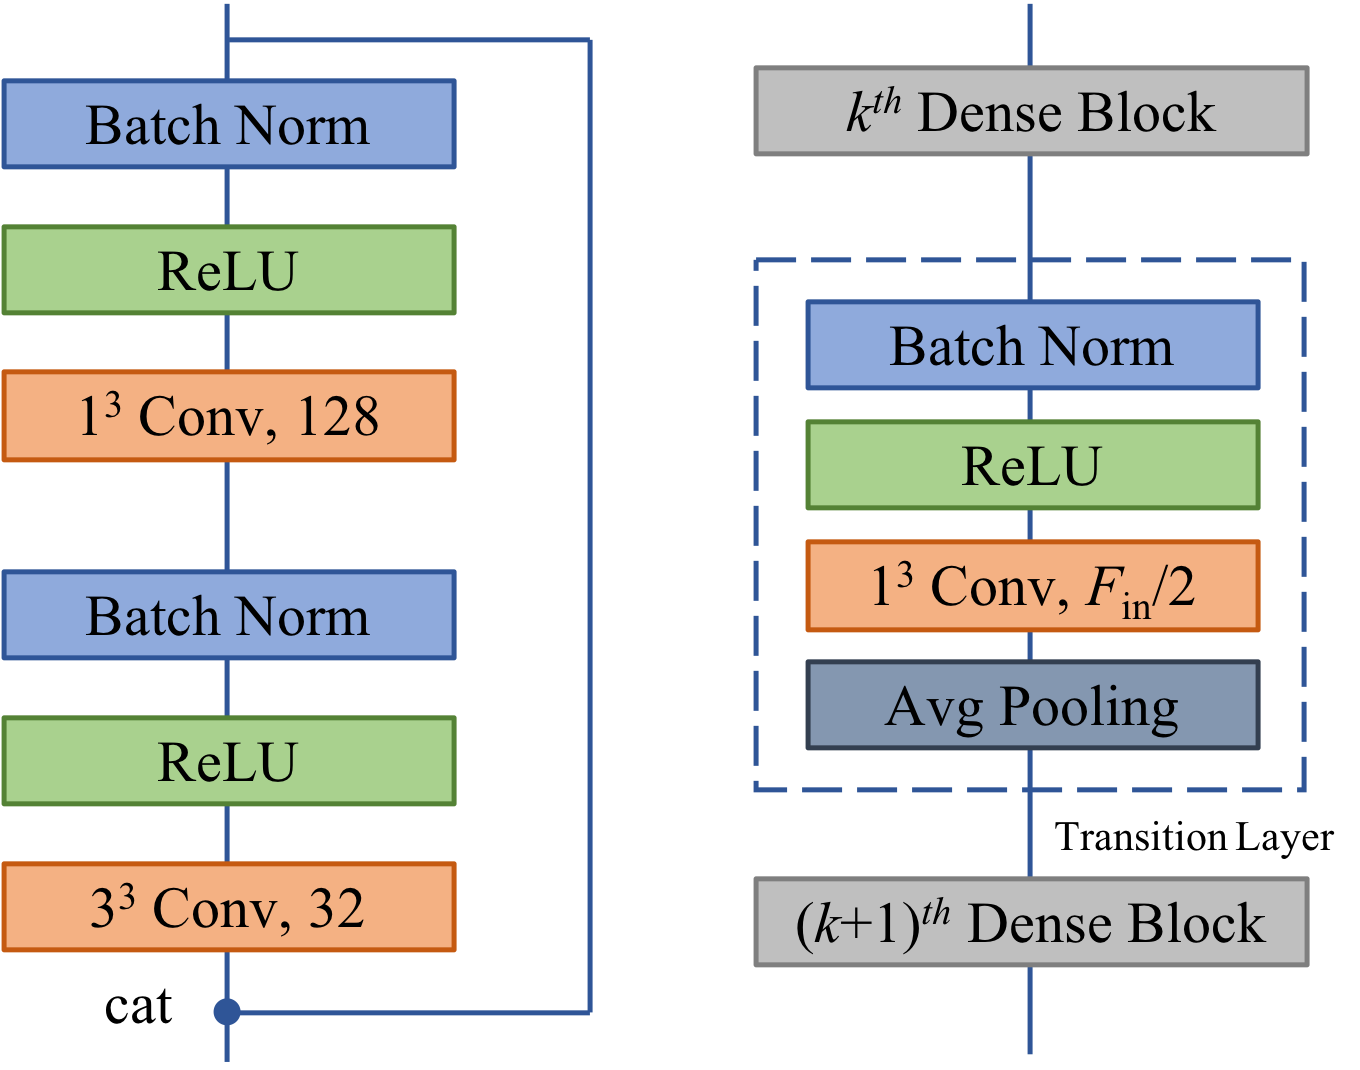
\includegraphics[scale=0.30]{fig/fig2.png}
\end{center}
\caption{Block diagram of bottleneck and transition layer in our model. The block [$x^3$ Conv, $F$] denotes a convolution layer that have the kernel size of $x \times x \times x$ and produces $F$ feature maps.}
\label{fig:bottleneck}
\end{figure}

\begin{table}
\begin{center}
\caption{Network architecture of the proposed method.}
\label{table:arch}
\begin{tabular}{lcr}
\hline
\textbf{Module Name} & \textbf{Architecture} & \textbf{Output Shape} \\
\hline\hline
Input Clip & - & [3,16,112,112] \\
Initial Conv & $7^3$ Conv, (1,2,2) & [64,16,56,56] \\
Pooling & $3^3$ Max & [64,8,28,28] \\
DenseBlock 1 & $(1^3, 3^3) \times 6$ & [256,8,28,28] \\
TransitionLayer 1 & $1^3$ Conv, $3^3$ Avg & [128,4,14,14]\\
DenseBlock 2 & $(1^3, 3^3) \times 12$ & [512,4,14,14] \\
TransitionLayer 2 & $1^3$ Conv, $3^3$ Avg & [256,2,7,7] \\
DenseBlock 3 & $(1^3, 3^3) \times 24$ & [1024,2,7,7]\\
GlobalAvgPooling & $2 \times 7 \times 7$ Avg & [1024,1,1,1]\\
Classification & FC Layer & [2,-,-,-] \\
\hline
\end{tabular}
\end{center}
\footnotesize
For $3^3$ convolution and pooling, the default stride is (2,2,2). The $(1^3, 3^3)$ denotes the bottleneck structure in Figure \ref{fig:bottleneck}.
\end{table}

%------------------------------------------------------------------------- 

\subsection{Bottleneck and Transition Layer}

Dense layer should be elaborately selected, since it is the basic component for processing useful feature maps. 
Here we adopt \emph{Bottleneck} architecture with pre-activation. 
The left diagram in Figure \ref{fig:bottleneck} represent the bottleneck structure of dense layers whose growth rate is 32 and bottleneck size is 4.
The kernel size of the first convolution layer is $1 \times 1 \times 1$ and that of the second convolution layer is $3 \times 3 \times 3$.
Typically, dense layer relatively at back may have more inputs as it receives all the feature maps from its preceding layers. 
Consequently, using bottleneck convolution helps to reduce the input feature maps, and thus improves computational efficiency.
Also, the expansion inside bottleneck promotes interaction between different channels, which is favorable for learning complex features.

Between any two dense blocks, we place a transition layer similar to \cite{densenet} in Figure \ref{fig:bottleneck}.
The main purpose of using transition layer is to down-sample the input feature maps and match the number of feature maps between adjacent blocks.
Here we set the number of output feature maps equal to half of the input number, as $F = F_{in}/2$. 
In addition to reducing the complexity and tuning the nonlinearity of the model, the transition layer can also help to promote interaction between channels, which enhances the feature learning ability and improves robustness of our model.

The internal details of the proposed model are listed in Table \ref{table:arch}. 
In Output Shape column, $[F, T, H, W]$ denotes the shape of output tensors (feature maps) produced by former module.
Note that dense blocks are slightly different from the simplified illustraion in Figure \ref{fig:model}. 


\begin{table*}
\begin{center}
\caption{Comparison of different methods on classification accuracy.}
\label{table:result}
\begin{tabular}{lccc}
\hline
\textbf{Method} & \textbf{Hockey Fights Dataset} & \textbf{Movies Dataset} & \textbf{VIolent Flows Dataset} \\
\hline\hline
Deniz et al. \cite{fast} & 90.1$\pm$0\% & 98.0$\pm$0.22\% & - \\
Bilinski et al. \cite{bilinski2016human} & 93.4\% & 99\% & 96.4\% \\
ViF + OViF \cite{ovif} & 87.5$\pm$1.7\% & - & 88$\pm$2.45\% \\
Substantial Derivative \cite{moha_avss} & - & 96.89$\pm$0.21\% & 85.43$\pm$0.21\% \\
MoIWLD \cite{MoIWLD} & 96.8$\pm$1.04\% & - & 93.19$\pm$0.12\% \\
\hline
Three streams + LSTM \cite{dong2016multi} & 93.9\% & - & - \\
FightNet \cite{zhou2017violent} & 97.0\% & 100\% & - \\
Hough Forests + CNN \cite{serrano2018fight} & 94.6$\pm$0.6\% & 99$\pm$0.5\% & - \\
ConvLSTM \cite{convlstm_sudh} & 97.1$\pm$0.55\% & \textbf{100$\pm$0\%} & 94.57$\pm$2.34\% \\
Bi-ConvLSTM \cite{bi_convlstm} & 98.1$\pm$0.58\% & \textbf{100$\pm$0\%} & 93.87$\pm$2.58\% \\
\textbf{Proposed} & \textbf{98.3$\pm$0.81\%} & \textbf{100$\pm$0\%} & \textbf{97.17$\pm$0.95\%} \\
\hline
\end{tabular}
\end{center}
\end{table*}

%------------------------------------------------------------------------ 

\section{Experiment and Analysis}

Several experiments have been conducted to evaluate the performance of the proposed model in terms of classification accuracy on three standard benchmark datasets. Meanwhile, computational efficiency of deep learning models is also considered and estimated.

\subsection{Dataset}

In violence detection tasks, there are three public standard benchmark datasets:

\textbf{Hockey Fights Dataset} \cite{hockey} contains 1000 videos collected from hockey games.
Each video consists of 50 frames with 720$\times$576 pixels. Nearlly all of the videos have the same background and human activities including fights and normal gamings.

\textbf{Movies Dataset} \cite{hockey} has 200 untrimmed video clips obtained from action movies with different resolutions. Different from Hockey, videos in Movies dataset vary in contents.

\textbf{VIolent-Flows Dataset} \cite{vif} consists of 246 videos of crowd behavior with frames resized to 320$\times$240 pixels.
Different perspectives, noisy background and dense crowd make this dataset relatively challenging for feature learning.

All of these three datasets contain balanced fight and non-fight samples. 
However, as designed for hand-crafted methods, these datasets are relatively small in scale, which may not be capable of training deep neural networks.
To cope with this problem, the ConvLSTM method \cite{convlstm_sudh} uses AlexNet model pre-trained on ImageNet.
Similarly, we consult the conclusion in \cite{3dcnn_2} and employ part of the parameters in their model which is pre-trained on Kinetics dataset \cite{kinetics}.
These parameters are imported to initialize the first convolutional layer in our model.

The three datasets are also mixed up as Mix dataset.
In Mix dataset, positive and negative samples are randomly drawn from original datasets separately in the same proportion.
Mix dataset can be used to evaluate overall performance for deep learning models of their modeling capability and generalization ability in violence detection task.

\subsection{Experiment Settings}

The proposed model is implemented using PyTorch \cite{pytorch} platform. 
When comparing inference speed, other deep models for comparision are also implemented with PyTorch to guarantee comparability and consistency.

The inputs of network are prepared as tensors with shape $N \times C \times T \times H \times W$, where $N$ is the batch size, $C$ is the number of channels (3 for RGB videos), $T$ is the duration of clips and $H \times W$ is the frame resolution. 
In the experiment, each video is extracted with 16 adjacent frames and then cropped and resized into 112$\times$112 pixels.

In the training phase, data augmentation is employed to enlarge training set and reduce overfitting, including random horizontal flipping, spatially random scale cropping and temporally random slicing. 
The learning rate and batch size are $10^{-3}$ and $32$ for Hockey and $10^{-4}$ and $16$ for Movie and ViF, considering the scales of dataset.
We apply mini-batch stochastic gradient descent (SGD) with momentum 0.5 and weight decay $10^{-3}$ for model optimization.  
Cross entropy function defined in \ref{eq:crossentropy} is used for loss calculation. 
\begin{equation}
\label{eq:crossentropy}
\operatorname{loss}(x, \text{label}) = -\log \left(\frac{\exp (x[\text{label}])}{\sum_{j} \exp (x[j])}\right)
\end{equation}

In the evaluation phase, videos in test set are spatially cropped around center position and temporally sliced to use centre adjacent frames.

For supplementary experiment on Mix dataset, we split it into training set and validation set with 9:1, as there are totally 1,446 videos. 
The proposed model is still trained by SGD algorithm with momentum, while ConvLSTM \cite{convlstm_sudh} model is optimized using RMSprop algorithm.
The batch size is set to 32 and learning rate is set to $10^{-3}$.

\subsection{Results and Discussion}

In the experiment, we adopt five-fold cross validation to evaluate the recognition performance of the proposed method to keep consistent with the previous methods.
Table \ref{table:result} gives the classification accuracy of the state-of-the-art methods on three standard datasets, with deep learning methods listed in the lower half of the table and hand-crafted methods in the upper half.
From this table, it can be seen that deep learning methods, generally perform better than hand-crafted methods.
Among them, the proposed method achieves the best performance on all of these three datasets.

As explained in Section \ref{sec:1}, violence is considered as aggressive behaviors of human. 
Consequently, it may be obscure to distinguish fights from ohter human body movements like sports and celebrations.
Taking Hockey Fights dataset for example, normal games can also contain body collision or powerful strokes, which can be confusing and have a real possibility to be mistaken as violence.
Nevertheless, the proposed model obtains the highest accuracy, implying that it is capable capturing spatiotemporal motion cues and high order localized region information. 
In the case of Movies dataset, since it has easily identifiable positive and negative samples, every model performs well.
As for VIolent-Flows dataset, dense crowd and noisy background make it challengeable to capture violent cues. 
Also, multi-scale and multi-viewpoint may be  another two factors that effect model performance.
Nevertheless, owing to the design of feature reusing and the global field of final decision, the proposed method forms a multi-attention mechanism for discovering violent position in videos.

%------------------------------------------------------------------------ 

\begin{table}
\begin{center}
\caption{Comparison of deep learning models on Mix dataset.}
\label{table:mix}
\begin{tabular}{lccc}
\hline
\textbf{Model} & \textbf{Accuracy} & \textbf{CE Loss} & \textbf{\# Params} \\
\hline\hline
C3D \cite{3dcnn_1} & 92.47\% & 0.4019 & 78.0M \\
ConvLSTM \cite{convlstm_sudh} & 96.58\% & 0.1355 & 9.6M \\
\textbf{Proposed} & \textbf{99.32\%} & \textbf{0.0326} & \textbf{7.4M} \\
\hline
\end{tabular}
\end{center}
\end{table}

\begin{figure}[t]
\begin{center}
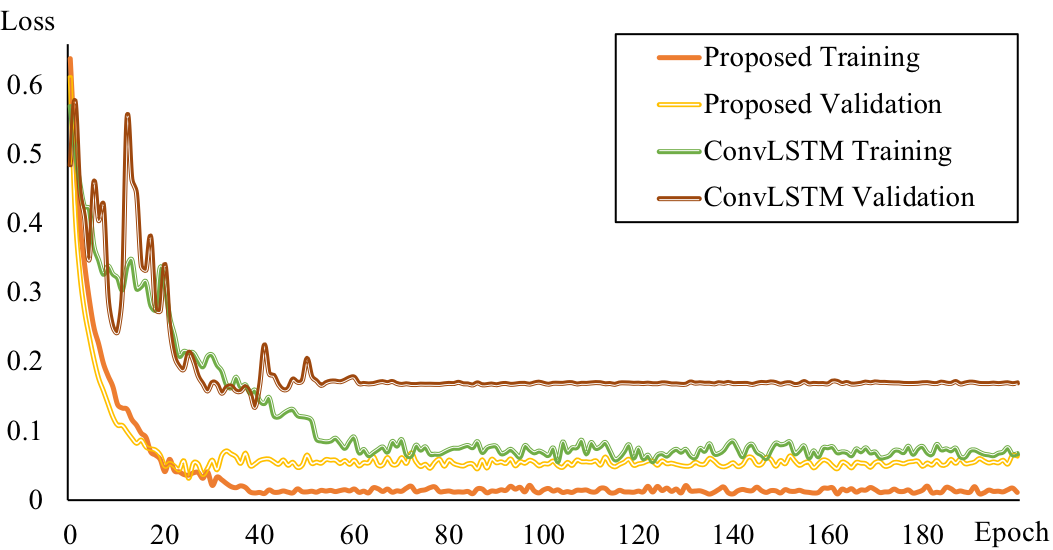
\includegraphics[scale=0.46]{fig/fig3.png}
\end{center}
\caption{Training and validation losses of the proposed model and ConvLSTM \cite{convlstm_sudh} on Mix dataset.}
\label{fig:mix}
\end{figure}

%------------------------------------------------------------------------ 

Supplementary experiment on Mix dataset is carried out to evaluate comprehensive performance of deep learning model.
Due to the limited conditions, we only evaluate our model with two classic methods, C3D \cite{3dcnn_1} and ConvLSTM \cite{convlstm_sudh}. 
As is given in Table \ref{table:mix}, the proposed model has better classification with relatively fewer parameters.
Its cross entropy loss on validation set is an order of magnitude lower than those of two other models.
Also, Figure \ref{fig:mix} illustrates the details of training and validation epochs. 
Compared to ConvLSTM, the proposed model is faster in convergence and more capable of modeling abstract features, with relatively lower validation loss.
This implies that the proposed model achieves better generalization and can effectively learn violence features.

%------------------------------------------------------------------------ 

\begin{table}
\begin{center}
\caption{Efficiency of deep learning models. The last three columns list the $n$-channel inference time per frame.}
\label{table:efficiency}
\begin{tabular}{lcccc}
\hline
\textbf{Model} & \textbf{FLOPS} & \textbf{1} & \textbf{8} & \textbf{16}\\
\hline\hline
C3D \cite{3dcnn_1} & 40.04G & \textbf{1.1ms} & 5.1ms & 9.9ms \\
ConvLSTM \cite{convlstm_sudh} & 14.40G & 3.7ms & 4.9ms & 6.3ms \\
\textbf{Proposed} & \textbf{10.43G} & 1.9ms & \textbf{3.6ms} & \textbf{5.7ms} \\
\hline
\end{tabular}
\end{center}
\end{table}

%------------------------------------------------------------------------

The effeciency of models is theoretically studied and practically estimated using torch.autograd.proflier library on single GTX 1080Ti.
Table \ref{table:efficiency} shows that the proposed model requires lower floating point operations (FLOPS) and is more computationally efficient.
Meanwhile, it has a faster inference speed and can process about 175 16-channel frames (i.e. 10$\times$16 video clips) per second.
However, as the architecture of our model require frequent memory I/O, it waste more time on small batch inputs. 
We will try to optimize its implementation and fix this problem in the future.
 
%------------------------------------------------------------------------

\section{Conclusions}
In this paper, we propose a deep learning model based on 3D convolutional neural networks with improved internal architecture. 
The proposed model has relatively fewer parameters and is more capable of learning spatiotemporal features in violent videos. 
Experiment results on three standard benchmark datasets demonstrate the improvement of our model compared to state-of-the-art methods. 
Also, the supplementary experiment on Mix dataset proves the effectiveness of our model's feature learning ability. 
At last, we evaluate the efficiency of several deep learning models from theoretical and practical aspects. 
Relatively, The proposed model saves more computing resources and is very efficient for real-time processing. 

In practical applications, sliding window strategy and voting mechanism can be adopted to achieve better recognition accuracies. 
By choosing a proper sample rate, it is accessible to make trade-offs between efficiency and accuracy for specific tasks.

{\small
\bibliographystyle{ieee}
\bibliography{egbib}
}


\rule{0pt}{1pt}\newpage


\end{document}
